% SEGMENT OLP-0635-S01
% Part: history
% Chapter: set-theory
% Section: limits

\documentclass[../../../include/open-logic-section]{subfiles}

\begin{document}

\olfileid{his}{set}{limits}

\olsection{எல்லைகளின் துல்லியமான வரையறை}

இன்றைய வழக்கில், மேலே கண்ட சிக்கலுக்கு நுண்ணளவுகளைக் கைவிடுவதே
தீர்வாக இருக்கிறது. அதை எப்படிச் செய்கிறோம் என்று பார்ப்போம்.

% SEGMENT OLP-0635-S02
% SOURCE CORRECTION TA-HIS-001: the varying difference quotient, not fixed f'(c), approaches the slope.
$\beta$ சிறிதாகும்போது சாய்வின் தோராயம் மேம்படுவதைக் கண்டோம்.
உண்மையில், $\beta$ ஆனது $0$-ஐ விரும்பிய அளவுக்கு அணுகும்போது,
வித்தியாச ஈவின் மதிப்பு நமக்குத் தேவைப்படும் சாய்வை நோக்கி
நெருங்குகிறது. எனவே $\beta = 0$ \emph{என்போது} என்ன நடக்கிறது என்று
ஆராய்வதற்குப் பதிலாக, $\beta$ ஆனது $0$-ஐ அணுகும்போது அந்த
ஈவின் \emph{நெருங்கும் போக்கையே} ஆராய்ந்தால் போதும்.

% SEGMENT OLP-0635-S03
இவ்வாறு பார்த்தால், பின்வரும் வடிவிலான கூற்றுகளுக்குத் துல்லியமான
பொருள் தருவதே பொதுவான சவால்:
\begin{center}
$x$ ஆனது $c$-ஐ அணுகும்போது, $g(x)$ ஆனது $\ell$-ஐ நோக்கி நெருங்குகிறது.
\end{center}
இதைச் சுருக்கமாக இவ்வாறு எழுதலாம்:
\[
\lim_{x \rightarrow c}g(x) = \ell.
\]
பத்தொன்பதாம் நூற்றாண்டில், கோஷியின் முந்தைய பணியை அடிப்படையாகக் கொண்டு,
வெயர்ஸ்ட்ராஸ் இந்தக் கூற்றுக்கு முற்றிலும் துல்லியமான வரையறையை
அளித்தார். $x$-ஐ $c$-க்கு ஏற்ற அளவு அருகில் எடுத்தால், $g(x)$-ஐ
$\ell$-க்கு நாம் விரும்பும் அளவுக்கு அருகில் கொண்டுவரலாம் என்பதே
கருத்து. இன்னும் துல்லியமாக, $\lim_{x \rightarrow c} g(x) = \ell$
என்பதன் பொருள் இதுவாகும்:
% SOURCE CORRECTION TA-HIS-002: ordinary limits use a punctured neighbourhood.
\[
(\forall\epsilon > 0)(\exists \delta > 0)\forall x \left(0 < |x - c| < \delta \lif |g(x) - \ell| < \epsilon \right).
\]
இது துளையிடப்பட்ட அண்மை: இங்கு அணுகப்படும் புள்ளி விலக்கப்படுகிறது;
அப்புள்ளியில் சார்புக்கு மதிப்பு இருக்க வேண்டிய அவசியமில்லை.

% SEGMENT OLP-0635-S04
இங்கு செங்குத்துக் கோடுகள் தனிமதிப்பைக் குறிக்கின்றன. அதாவது,
$x \geq 0$ எனில் $|x| = x$; $x < 0$ எனில் $|x| =-x$.
\emph{இந்தச்} சார்பை இவ்வாறு வரையலாம்:
\begin{center}
	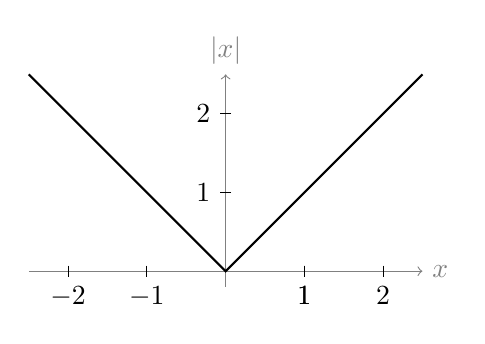
\begin{tikzpicture}[scale=1]
	\draw[->, gray] (-2.5,0) -- (2.5,0) node[right] {$x$};
	\draw[->, gray] (0,-.2) -- (0,2.5) node[above] {$|x|$};

	\foreach \x/\xtext in {-2/-2, -1,1, 1/1, 2/2}
	\draw[shift={(\x,0)}] (0pt,2pt) -- (0pt,-2pt) node[below] {{$\xtext$}};

	\foreach \y/\ytext in {1/1, 2/2}
	\draw[shift={(0,\y)}] (2pt,0pt) -- (-2pt,0pt) node[left] {{$\ytext$}};

	\draw[thick] (-2.5, 2.5)--(0,0)--(2.5, 2.5);
	\end{tikzpicture}
\end{center}
ஆகவே, வரையறையின் தோராயமான பொருள் இதுதான்: $c$-இலிருந்து
$\delta$-ஐவிடக் குறைந்த தூரத்திலுள்ள உள்ளீடுகளைத் தேர்ந்தெடுத்தால்
(அதாவது, $|x -
c| < \delta$), உங்கள் “பிழையை” $\epsilon$-ஐவிடக்
குறைவாக (அதாவது, $|g(x) - \ell| < \epsilon$) ஆக்கலாம்.

% SEGMENT OLP-0635-S05
எல்லை என்ற கருத்தை வரையறுத்துவிட்டதால், நுண்ணளவுகளை முற்றிலும்
தவிர்க்கலாம். $c$-இல் $f$ சார்பின் சாய்வு பின்வருமாறு தரப்படுகிறது:
\[
	{f}'(c) = \lim_{x \rightarrow 0}\left(\frac{f(c +x) - f(c)}{x}\right) \text{ எல்லை இருந்தால்}.
\]
“எல்லை இருந்தால்” என்ற வரம்பு ஏன் தேவை என்பதை உணர்வது முக்கியம்.
எளிய எடுத்துக்காட்டாக, இப்போதுதான் வரைபடம் பார்த்த $f(x) = |x|$
என்ற சார்பை எடுத்துக்கொள்ளுங்கள். இங்கே $f'(0)$ வரையறுக்கப்படவில்லை:
$0$-ஐ “வலப்புறத்திலிருந்து” அணுகினால் சாய்வு எப்போதும் $1$;
$0$-ஐ “இடப்புறத்திலிருந்து” அணுகினால் சாய்வு எப்போதும் $-1$.
எனவே எல்லை இல்லை. இத்தகைய எல்லை இருந்தால், இருந்தால் மட்டுமே,
ஒரு சார்பு~$f$, புள்ளி~$x$-இல் \emph{வகையிடத்தக்கது} என்று கூறலாம்.

% SEGMENT OLP-0635-S06
\emph{எல்லை} என்ற கருத்தைப் பயன்படுத்தி வகையிடலை எப்படிக்
கையாளலாம் என்று கண்டோம். அதே கருத்தைக் கொண்டு \emph{தொடர்ச்சியான}
சார்பு~$f$-ஐயும் வரையறுக்கலாம். (1817-ஆம் ஆண்டுக்குள் போல்சானோ இதைச்
சாராம்சத்தில் உணர்ந்திருந்தார்.) தொடர்ச்சியைப் பற்றிய கோஷி--வெயர்ஸ்ட்ராஸ்
விளக்கம் இதுதான். பொதுவாகச் சொன்னால், ஒரு சார்பின் வெளியீட்டில்
ஒரு குறிப்பிட்ட துல்லியத்தை விரும்பினால், அதன் உள்ளீட்டில்
போதுமான துல்லியத்தை வலியுறுத்தி அதை உறுதிசெய்ய முடியும் எனில்,
அந்தச் சார்பு ஒரு புள்ளியில் தொடர்ச்சியானது. இன்னும் துல்லியமாக,
$x$ பூச்சியத்தை அணுகும்போது $f(c + x)$-க்கும் $f(c)$-க்கும்
இடையிலான வேறுபாடும் $0$-ஐ அணுகினால், $f$ சார்பு $c$-இல்
தொடர்ச்சியானது. வேறு விதமாகச் சொன்னால், $f(c) = \lim_{x \rightarrow c} f(x)$
எனில், எனில் மட்டுமே, $f$ ஆனது $c$-இல் \emph{தொடர்ச்சியானது}.

% SEGMENT OLP-0635-S07
இதற்கு மேல் சென்றால், நமது பொருளான கணக் கோட்பாட்டை விட்டு மெய்யெண்
பகுப்பாய்வுக்குச் சென்றுவிடுவோம். எனவே இங்கே நின்று இந்தப் பாடத்தின்
கருத்தைச் சொல்லலாம். பத்தொன்பதாம் நூற்றாண்டில் கணிதவியலாளர்கள்,
துல்லியமாக வரையறுக்கப்பட்ட \emph{எல்லை} என்ற கருத்தைப் பயன்படுத்தி
நுண்ணளவுகள் இன்றியே செயல்படக் கற்றுக்கொண்டனர்.

\end{document}
